\pdfoutput=1

\documentclass[11pt]{article}

\usepackage[final]{final}
\usepackage{times}
\usepackage{latexsym}
\usepackage[T1]{fontenc}
\usepackage[utf8]{inputenc}
\usepackage{microtype}
% \usepackage{inconsolata}
\usepackage{graphicx}
\title{Efficient Image Compression}

\author{James Camacho \\
  MIT / AI \\
  \texttt{jamesc03@mit.edu} \\\And
  Linda He \\
  Harvard / Applied Mathematics \\
  \texttt{lindahe@college.harvard.edu} \\}

\begin{document}
\maketitle
\begin{abstract}
  With high-dimensional spaces such as images or video, perfect communication becomes prohibitively expensive. A lossy, compressed version is cheaper to transmit and often good enough for most purposes. Traditional algorithms such as JPEG use a Fourier transform to pick out the most important features for transmission. In this paper, we explore using auto- and raster-encoders to automatically and efficiently compress images instead. We find they significantly outperform JPEG on the MNIST dataset, and discuss potential future improvements to their speed and cost via reinforcement learning.
\end{abstract}


\section{Introduction}

Over 75\% of internet traffic comes in the form of video \citep{cisco-2018-traffic}, and YouTube alone nets \$30bn from their distribution \citep{alphabet-2024-earnings}. At these massive scales, every extra bit of compression is important. In this paper, we explore more optimal compression with the use of deep learning methods, including one adapted from language models.

Image and text have often been treated as separate domains, but there is much that can be applied between the two. Inspired by quantization and fractalization from image compression, Witten \textit{et al.} proposed several lossy text encoding schemes as far back as 1992 \citep{witten-etal-1992-lossy}. Recent advances in image generation such as denoising models \citep{ho-2020-denoising} have similarly found applications in text generation by directly translating pixels into language tokens \citep{kou-2024-cllms}. Going the other direction, the popular Transformer architecture of language models have been applied to vision \citep{dosovitskiy-2021-vit}, and has seen state-of-the-art success in video production \citep{liu-2024-sora}.

As we will see in \ref{sec:jpeg}, the Vision Transformer algorithm bears a striking resemblance to JPEG. This is no accident. Generation is the inverse of compression, and more generally ``being able to compress well is closely related to acting intelligently'' \citep{hutter-2020}. Unfortunately, this enforces a tradeoff between the algorithm's speed and size. For example, an unintelligent compressor may store images verbatim, or a generator may simply sample from its training dataset. Smarter algorithms will do much better, but require more computation.

This paper will focus on the tradeoff between image quality and compression length, but we will end with several suggestions for improving the running time via reinforcement learning.


\section{Related Work}

\section{Methods}

\subsection{JPEG}\label{sec:jpeg}

These vision transformers bear a striking resemblance to the JPEG algorithm

\subsection{Auto-Encoders}

Reference the paper about how CNNs find features like stripes.

\begin{figure*}[t]
  \centering
  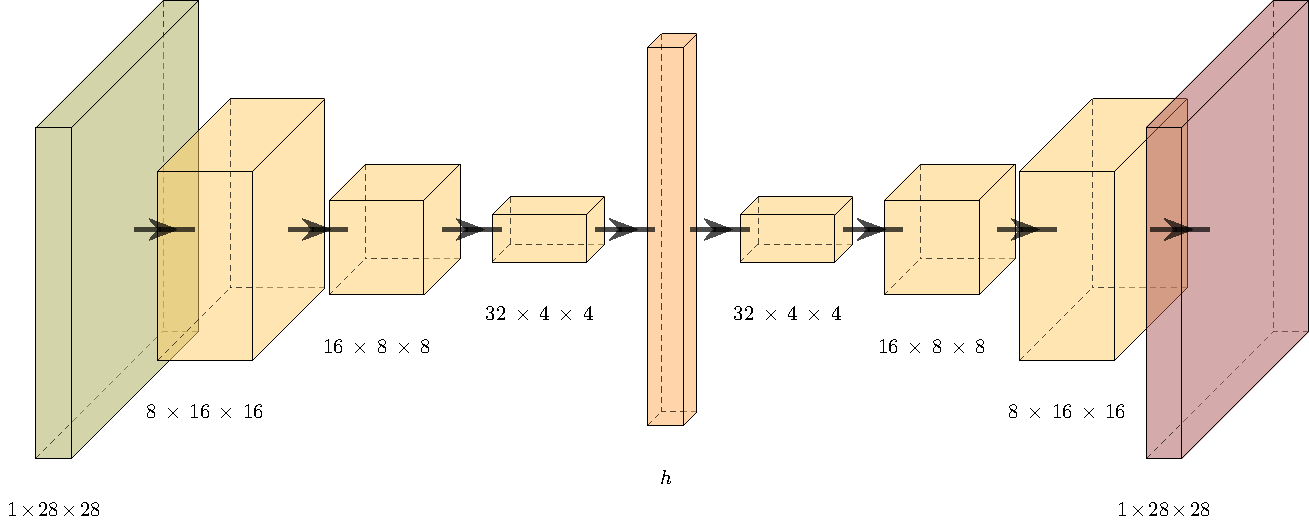
\includegraphics[width=2\columnwidth]{diagrams/auto.pdf}
  \caption{Auto-encoder network.}
  \label{fig:auto}
\end{figure*}

\subsection{Raster-Encoders}

\begin{figure*}[t]
  \centering
  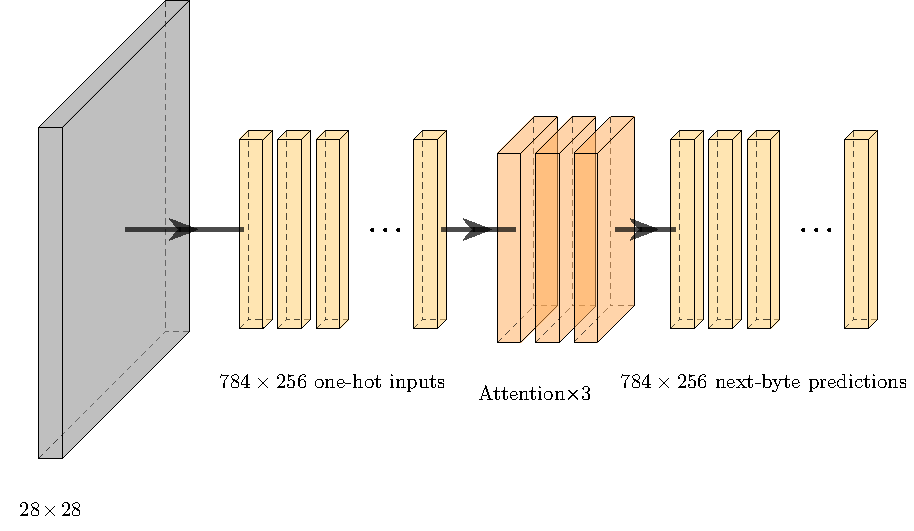
\includegraphics[width=2\columnwidth]{diagrams/raster.pdf}
  \caption{Raster-encoder network.}
  \label{fig:auto}
\end{figure*}


\section{Discussion}

Testing this: This is some text with a citation \citep{lazaridou-etal-2020-multi}.

\section*{Acknowledgments}

\bibliography{references}

\appendix

\section{Example Appendix}
\label{sec:appendix}

This is an appendix.

\end{document}
